\documentclass{article}
\usepackage{arxiv}
\usepackage{ctex}
\usepackage{CJK}
\usepackage{enumerate}
\usepackage[T1]{fontenc}    % use 8-bit T1 fonts
\usepackage{hyperref}       % hyperlinks
\usepackage{url}            % simple URL typesetting
\usepackage{booktabs}       % professional-quality tables
\usepackage{amsfonts}       % blackboard math symbols
\usepackage{nicefrac}       % compact symbols for 1/2, etc.
\usepackage{microtype}      % microtypography
\usepackage{lipsum}		% Can be removed after putting your text content
\usepackage{graphicx}
\usepackage{caption}
\usepackage{geometry}
\usepackage{multirow}
\usepackage{array}
\usepackage{longtable}
\usepackage{booktabs}
\usepackage{indentfirst}
\usepackage{tikz,mathpazo}
\usepackage{flowchart}
\usepackage{float}
\usepackage{subfigure}
\usepackage{mathrsfs}
\usepackage{amsfonts}
\usepackage[linesnumbered,boxed,ruled,commentsnumbered]{algorithm2e}
\usetikzlibrary{arrows,shapes,chains}
\setlength{\parindent}{2em}
\setlength{\abovecaptionskip}{0cm}
\setlength{\belowcaptionskip}{-0.25cm}
\title{双渠道绿色供应链博弈模型的稳定性研究}
\author{
    吴俊达\\数学与统计学院\\统计与精算系\\joshua19801010@gmail.com\\
    \And
    杨帆\\数学与统计学院\\应用数学系\\fany02656@gmail.com
    \And
    刘芝延\\数学与统计学院\\应用数学系\\
}

\begin{document}
\maketitle
\begin{abstract}
本文研究了一类双渠道绿色供应链博弈模型,在传统模型的基础上,增加了产品的绿色环保等级参数$\theta$。考虑了政府环保政策对绿色产品的价格补贴,以及政府对于绿色产品生产的成本优惠因素。我们建立了一个由厂商主导的Stackelberg主从式博弈模型,同时完成了对其的静态系统和动态系统的数学建模。我们求解了博弈模型的几个均衡解,分析了其各自的稳定性和稳定区间。通过我们自己开发的混沌分析工具,通过大规模的数值模拟方法,我们分别求解得到了针对以上两个因素的系统分岔路径和Lyapunov指数图。我们讨论了对于$\theta$,线性的价格补贴因子$\lambda$和二次成本优惠因子$\eta$,在双方价格调整能力相同和相异两种情形下的影响。模拟结果表明,上述两种激励手段,对于厂商主导主动提高其商品环保等级起到积极作用,激励力度与产品绿色等级成正相关。然而,当激励力度超过一定水平(有市场的特征决定),双渠道博弈将会逐步出现混沌,且在某一小区间($\delta$邻域)将出现“线上线下”恶性价格竞争的情况。从另一方面,在价格调控能力相当的假设下,线下零售商的利益将完全消失,即批发价等于零售价,呈现被直销渠道替代的态势,这和近年来的消费市场形势类似。在加入环保因素考虑后,在某一参数区间下,零售商的利润空间将重新出现,但是其Lyapunov指数持续大于批发价,即不稳定程度较大。我们认为这类所谓环保因素的考虑,可类比推广到各类附加值产品供应链模型中。这类附加值因素有利于线下零售商重新获得议价能力和市场空间,但是在厂商主动的博弈模式下,零售商所面对的不确定性依然大于厂商。该研究结果也表明,政府激励手段的过度干预,会显著的增大市场的不确定性以及混沌程度。
\end{abstract}
\keywords{绿色供应链,Stackelberg博弈,分岔路径,Lyapunov指数,政策激励}
\newpage
\section{介绍}
\par \textbf{note1: 问题的研究背景,双渠道供应链背景(电商、厂商),关于经济学的定性研究结论。}
\par 传统的双渠道供应链模型包括一个制造商和一个传统经销商的博弈模式。然后近年来许多学者从实际生产生活中抽象出多种模型,并分别进行了建模和均衡的求解。Wang等(2016)\cite{2016Wang}研究了厂商增加电商和第三方直销这两种额外渠道,分别对传统博弈结果的影响。Zhao(2017)\cite{2017Zhao}等人求解了两个制造商和一个经销商的情况。Xie(2018)\cite{2018Xie}等人综合前人研究增加了厂商和经销商的一致模式,并给出了完整的数学求解。Arshad(2018)\cite{2018Arshad}等人讨论了两个经销商的合作对抗厂商的博弈策略,并加入商品回收机制,考虑闭环供应链。Pathak、Giri和Hosseini-Motlagh等(2019)\cite{2019Pathak}\cite{2019Giri,2019Hosseini-Motlagh}都研究了闭环供应链模型中回收商的组织和回收价格对博弈策略的作用,并且讨论了参数对于均衡点稳定性的影响。王虹等(2009)\cite{2009Wang}讨论了一致与非一致下的Stackelberg博弈模型,认为厂商的决策在非一致模式下优于一致模式。Li等(2016)\cite{2016Li}研究了非一致模式下考虑公平因素的Stackelberg博弈,认为经销商会在已知不对等的地位下,通过降低价格来获取市场份额的增加。Wang(2018)\cite{2018Wang}等人讨论了一致模式和非一致Bertrand模式下引入公平考虑的作用。Dai等(2019)\cite{2019Dai}进一步进行了同样的建模求解,进一步给出了参数显著性的分析。
\par 这一类动态博弈模型,以及其演化模式,通常描述为一个动力系统模型。因此运用动力学分岔理论研究博弈系统的稳定性成为主流研究方法。唐兴巧等(2017)\cite{2017Tang}利用数值模拟系统的分岔图等动力学特征分析了了系统Nash均衡点的稳定性,并得出了系统存在混沌行为导致市场不规律的后果。张芳等(2018)\cite{2018Zhang}和Zhang等(2015)\cite{2015Zhang}分别在公平因素条件下和闭环系统条件下,利用同样的工具研究动力系统的Hopf分岔图、Lyapunov指数以及混沌引子等指标。Li等人在2018年,通过一系列问题的实证研究,将该方法运用到了各个博弈场景中\cite{2018Huang,2018Qiu-Xiang,2019Qiu-Xiang1,2019Qiu-Xiang2}。
\par \textbf{note2: 绿色供应链和制度约束(ECSC)\cite{2005Beamon}。}Sheu等(2012)\cite{2012Sheu}的研究发现,当政府基于环保因素考虑,通过财政手段对供应链主体征税以及补贴,供应链博弈均衡的收益和社会福利都有显著的提高。进一步,Sinayi等(2018)\cite{2018Sinayi}和Aslani等(2019)\cite{2019Aslani}引入了消费者对绿色产品的线性倾向性需求,同时考虑制造商生产绿色产品的额外成本,研究政府的各类干预措施分别的有效性。Rahmani等(2018)\cite{2018Rahami}研究了需求扰动下的双渠道绿色供应链的定价模式。
\par 本文的工作主要分为三个部分:模型的建立、稳定性分析、得出的结论。第二节中我们采用了主流文献中讨论的,基于环保税的线性惩罚项(主要形式为征税和补贴),以及厂商主动额外附加的生产环保产品的二次项成本,对基础的博弈模型和动力系统模型进行修改。第三节中,我们主要完成了传统双渠道供应链Stackelberg博弈模型,以及其动力系统模型的建立。并对模型进行均衡点求解,用分析的方法解释其稳定性。进而在第四节,我们利用数值方法,完成了基于环保参数的演化分析,给出度量混沌效应的Hopf分岔图和最大Lyapunov指数图。在这一节中,我们验证了政府基于环保考虑对博弈均衡以及供应链收益的影响。同时,通过对比制度约束下系统稳定性状况,试图阐述政府对该类型供应链的制度监管对行业发展健康程度的影响。最后一节,我们将从经济和社会的层面,试图重新解释我们得出的结果。本文的创新点主要在以下:%电动汽车补贴
\begin{itemize}
    \item 在绿色供应链的研究中,文献主要集中于成本、固定税率以及绿色产品的受欢迎程度上。我们引入了与绿色程度线性相关的政府补贴因素,作为绿色产品的附加竞争力描述。
    \item 我们完成了双渠道绿色供应链的建模求解,同时创新地分析了环保制度对于供应链的稳定性影响。在经济和社会的层面,我们的研究可以一定程度下填补制度设计对市场稳定性考虑的不足。
    \item 在系统混沌分析方面的工作,我们主要依赖于数值模拟的研究方法,该方法对于模型表达式的微分性质等要求较低。同时在计算Lyapunov指数的工作中,我们不同于大多数论文中基于特征矩阵(Jacobi矩阵)的解析算法,利用了其原始定义,并通过大样本模拟迭代的基础下完成求解。该方法易于推广到更复杂的,以及无法显式求解的模型中去。
    \item 在数值计算方面的工作,我们不再依赖常用的matlab工具包。我们编写了针对三个博弈目标(可非常容易地扩展到多个)的动力系统混沌分析python工具包,计算Hopf分岔轨迹以及模拟计算Lyapunov指数。基于混沌分析模拟的可并发性,我们主要支持基于cuda计算库和Nvidia GPU的高速计算。实验在GeForce 980M的环境下,完成了每秒约$2\times10^5$个样本,每个样本1000次的迭代计算。(GitHub: JoshuaWu1997/chaos-analysis.git)
\end{itemize}
\section{问题描述与模型建立}
\par 本文考虑简单的双渠道供应链模型,其中包含一个供应商和一个一级零售商。供应商生产商品,分别通过批发给零售商以及通过直销渠道卖给顾客获利。零售商则从供应商进货,转卖给顾客获利。顾客则存在直销和进销商两个渠道购得商品。我们通过对市场的基本假设,固定了二者无需博弈的因素。同时我们引入了第三方监管力度的参量。我们的建模如下:
\par \textbf{基本假设一:}我们考虑线性的供需关系,其中固有需求$\alpha$边际需求与边际替代率假设相同$\beta$,即认为两种渠道的商品完全一致,没有差别,并且直销价格和经销商售价一致为$p$\cite{2016Li}。在绿色供应链中,假设只存在一种绿色商品,其绿色程度$\theta$系数直接影响受到顾客额外的欢迎程度和生产成本\cite{2012Ghosh}。从而,该统一价格的双方市场需求分别为:
\begin{equation}
    D_r=\alpha-\beta p+\lambda_r\theta
\end{equation}
\begin{equation}
    D_m=\alpha-\beta p+\lambda_m\theta
\end{equation}
\par 其中$\lambda_r, \lambda_m$分别度量了消费者对不同渠道相同绿色产品的不同认同度。
\par \textbf{基本假设二:}我们考虑政府对拥有不同$\theta$的商品进行价格补贴$\tau$。Sinayi(2018)也在其模型中加入了一次性的影响,即附加一个固定的价格补贴\cite{2018Sinayi}。基于现实政策中,逐渐出现更为灵活的,基于绿色程度的奖惩制度,于是我们创新地引入了与$\theta$线性相关的补贴项。由于方程的线性性质,该影响又可以被看作是在消费者角度,通过价格优势形成的额外需求。从而与消费者主观偏好系数$\lambda$可被统一归因为同类型影响,即:
\begin{equation}
    D_r=\alpha-\beta (p-\tau\theta)+\lambda_r\theta=\alpha-\beta p+(\lambda_r+\tau)\theta
\end{equation}
\begin{equation}
    D_m=\alpha-\beta (p-\tau\theta)+\lambda_m\theta=\alpha-\beta p+(\lambda_m+\tau)\theta
\end{equation}
\par \textbf{基本假设三:}我们假设制造商制造绿色商品的额外成本与$\frac{\theta^2}{2}$相关,系数$\eta$。制造商批发给零售商的价格$w$低于售价$p$,高于其基础成本$c$。则二者的收益(效用)可被表示为\cite{2012Ghosh}\cite{2016Li}:
\begin{equation}\label{U_m}
    U_m(p,w,\theta)=\pi_m=(w-c)(\alpha-\beta p+\lambda_r\theta)+(p-c)(\alpha-\beta p+\lambda_m\theta)-\eta\frac{\theta^2}{2}
\end{equation}
\begin{equation}\label{U_r}
    U_r(p,w,\theta)=\pi_r=(p-w)(\alpha-\beta p+\lambda_r\theta)
\end{equation}
\par \textbf{基本假设四:}基于Stackelberg博弈模型,该供应链的批发价格$w$以及商品的绿色程度$\theta$先由供应商确定。其后,零售商通过调整销售价格来达到自己利益的最大化\cite{2009Wang},此时基于假设一,直销渠道价格必须跟随。同时,政府可以通过调控价格补贴参数$\lambda$和成本系数$\eta$来调控市场。
\section{均衡求解}
\par 在基于Stackelberg假设下,供应商首先做出反应,供应商可以同时调整批发价格$w$和绿色程度$\theta$来使得自己的利益最大化。在给定的市场价格$p$的情况下,供应商的边际效用(效用函数的梯度)为:
\begin{equation}
    \frac{\partial U_m}{\partial w}(w;p,\theta)=\alpha-\beta p+\lambda_r\theta
\end{equation}
\begin{equation}
    \frac{\partial U_m}{\partial \theta}(\theta;p,w)=(w-c)\lambda_r+(p-c)\lambda_m-\eta\theta
\end{equation}
\par 同理可得零售商对于供应商给出的$w,\theta$做出反应,调整市场价格,其边际效益为:
\begin{equation}
    \frac{\partial U_r}{\partial p}(p;w,\theta)=\alpha-\beta (2p-w)+\lambda_r\theta
\end{equation}
\par 在实际博弈场景下,由于有限理性的约束,博弈双方只能在当前状态下做出能力范围内的调整,是的自己的收益向更优的方向发展。此时,假设博弈目标$p, w, \theta$相对应的每次调整能力固定为$k_p, k_w, k_\theta$,则可构建动态博弈模型,即时间离散的动力系统:
\begin{equation}\label{iteration}
    \left\{  
        \begin{array}{lr}
            w(t+1)=w(t)+k_ww(t)[\alpha-\beta p(t)+\lambda_r\theta(t)]               \\  
            p(t+1)=p(t)+k_pp(t)[\alpha-2\beta p(t)+\lambda_r\theta(t)+\beta w(t)]   \\  
            \theta(t+1)=\theta(t)+k_\theta\theta(t)[\lambda_rw(t)+\lambda_mp(t)-\eta\theta(t)-c(\lambda_r+\lambda_m)]
        \end{array}  
    \right.
\end{equation}  
\par 在Stackelberg博弈中,零售商只能被动的接受厂商事先设定的$w, \theta$,之后对于自己的调控的参数$p$做最优化的选择。同时厂商需要在已知零售商做出的零售价决定后,调整自己生产的参数 $\theta$和批发价$w$来使得自己利润最优化。所以,以下我们站在双方的角度,分别求解。
\subsection{厂商的角度}
\par 厂商需要在零售商确定零售价$p$的前提下,对自我的效用最优化,而零售价则是由零售商效用最大化决定的,即:
\begin{equation}\label{p_star}
    p^*(w,\theta)=\frac{\alpha+\lambda_r\theta+\beta w}{2\beta}
\end{equation}
\par 此时的厂商的效益最大化,可看作厂商内部的最优化问题,因为市场价格与自身生产的关系已知,将式(\ref{p_star})带入式(\ref{U_m})得到厂商效益:
\begin{equation}
    U_m^*(w,\theta)=\frac{1}{2}(w-c)(\alpha+\lambda_r\theta-\beta w)+\frac{1}{2}(\alpha+2\lambda_m\theta-\lambda_r\theta-\beta w)(\frac{\alpha+\lambda_r\theta+\beta w}{2\beta}-c)-\eta\frac{\theta^2}{2}
\end{equation}
\par 为了求解其均衡点,我们不妨令$\beta=1, \lambda_r=\epsilon\lambda_m$,简化求解过程,得到Nash均衡点方程:
\begin{equation}  
    \left\{  
        \begin{array}{lr}
            \lambda_r\theta-3\epsilon w+\epsilon\alpha+2\epsilon c=0               \\  
            \lambda_rw-2\epsilon\eta\theta+2\lambda_r\alpha-2\lambda_rc=0   
        \end{array}  
    \right. 
\end{equation} 
\par 得到了Nash均衡点和有界均衡点分别为:$E_1=(0,0)$, $E_2=(\frac{\alpha+2c}{3},0)$, $E_3=(0,\frac{\lambda_r(\alpha-c)}{\epsilon\eta})$, $E^*=(w^*,\theta^*)$,其中:
$$\theta^*=\frac{\epsilon\lambda_r(4c-7\alpha)}{\lambda_r^2-6\epsilon^2\eta},\quad
w^*=\frac{2\lambda_r^2(\alpha-c)+2\epsilon^2\eta(\alpha+2c)}{\lambda_r^2-6\epsilon^2\eta}$$
\par 我们利用Jacobi矩阵的性质来判别这些均衡点的稳定性\cite{2017Tang}\cite{2018Li},首先对于$E_1$有:
\begin{equation}\label{jacobi_1}
    J(E_1)=
    \left[
    \begin{array}{ccc}
        1+\frac{\alpha}{2}k_w&0&0\\
        0&1&0\\
        0&0&1+\frac{\alpha-2\epsilon c-2c}{2\epsilon}\lambda_rk_\theta
    \end{array}
    \right]
\end{equation}
\par 由式(\ref{jacobi_1})可得$J(E_1)$的特征值为:$\lambda_1=1+\frac{\alpha}{2}k_w$,$\lambda_2=1$,$\lambda_3=1+\frac{\alpha-2\epsilon c-2c}{2\epsilon}\lambda_rk_\theta$。已知各系数均大于零,根据判别法则可知,$|\lambda_1\lambda_2\lambda_3|>1$,即该均衡点不稳定,同理可将非Nash均衡点代入计算得边界均衡点都是不稳定的。以下,计算Nash均衡点的Jacobi矩阵:
\begin{equation}
    J(E^*)=
    (1+k_wh_1)(1+k_ph_2)(1+k_\theta h_3)
    \left[
    \begin{array}{ccc}
        \frac{1+k_wh_1}{k_ww^*} & -\beta & \lambda_r \\
        \beta & \frac{1+k_ph_2}{k_pp^*} & \lambda \\
        \lambda_r & \lambda_m & \frac{1+k_\theta h_3}{k_\theta\theta^*}
    \end{array}
    \right]
\end{equation}
\par 其中$h_1=\alpha-p^*+\lambda_r\theta^*$,$h_2=-\alpha-\lambda_r\theta^*-w^*$,$h_3=(1+\frac{1}{2\epsilon})\lambda_rw^*+(\frac{\lambda_r^*}{2\epsilon}-2\eta)\theta^*+(\frac{\alpha-2c}{2\epsilon}-c)\lambda_r$。对于该矩阵的特征值分析过于复杂,我们依然沿用前人的计算经验,套用了Jury判别条件\cite{2017Tang}。则该系统在Nash均衡点稳定的充分必要条件为:
\begin{equation}\label{jury}
    \Omega^*=
    \left\{
    \begin{array}{rl}
        1+Tr+Det>0 \\
        1-Tr+Det>0 \\
        1-Det>0
    \end{array}
    \right.
\end{equation}
\par 其中$Tr$和$Det$分别表示Jacobi矩阵的迹和特征值,通过计算得到该系统的稳定性条件。
\begin{equation}\label{tr_det}
    \left\{
    \begin{array}{l}
        Tr=3+k_wh_1+k_ph_2+k_\theta h_3 \\
        Det= (1+k_wh_1)(1+k_ph_2)(1+k_\theta h_3)(\frac{\beta^2}{1+k_\theta h_3}-\frac{\lambda_r^*2}{1+k_ph_2}-\frac{\lambda_r\lambda_m}{1+k_wh_1})
    \end{array}
    \right.
\end{equation}
\par 将式(\ref{tr_det})代入式(\ref{jury})则可得到Nash均衡点附近的稳定区域,该区域是由参数的选择所决定的。
\subsection{经销商的角度}
\par 经销商需要在厂商确定批发价$w$和绿色等级$\theta$的前提下,对自我的效用最优化,而这二者则是由厂商商效用最大化决定的,即:
\begin{equation}\label{t_star}
    \theta^*=\frac{\lambda_rw+\lambda_mp-(\lambda_r+\lambda_m)c}{\eta}
\end{equation}
\par 对于厂商批发价边际价格的讨论,我们发现:在一步博弈下,厂商批发价的制定并不受限,即:
\begin{equation}\label{w_star}
    \frac{\partial U_m}{\partial w}=\alpha-\beta p+\lambda_r\theta^*>0
\end{equation}
\par 此时的经销商的效益最大化,然而厂商如何决定制定自己的批发价我们难以在此确定。因为,在任何一步博弈下,当经销商确定了市场价格,厂商都可以通过一种霸道的策略,即将批发价定制的高于售价,使零售商无利可图从而退出市场,并且这种情况在实际中确实存在。然而,长期博弈中,由于某些外部因素,二者可以博弈形成一种可持续的合作关系。
\section{稳定性的数值分析}
\par 数值分析模拟动力系统演化模式是一种非常直观有效的工具。在本文所描述的系统中,我们重点关注外部影响,包括政府对绿色原料的补贴($\eta$),以及对绿色产品的支持力度($\lambda_r, \lambda_m$),对双方博弈路径的影响,以及其中可能产生的混沌现象。而我们研究的目标即为双方的博弈目标:批发价$w$,零售价$p$和绿色等级$\theta$。对动力系统混沌性的描述,我们采用了文献中普遍采用的二维分岔图,以及Lyapunov指数\cite{2017Tang}\cite{2018Zhang}\cite{2015Zhang}\cite{2018Huang}。除上述研究因素以外,我们不失一般性的对余下的参数预先赋值,简化模型计算成本,同时提出以下假设:
\par \textbf{基本假设五:}在以下的模拟计算中,我们假设$\alpha=3, \beta=1, c=1$。我们认为绿色产品在直销渠道的吸引力较弱于经销渠道,假设这种差异为一个较小的常数(否则二者竞争差异过大,系统在很早的时候就会发生崩溃),即$\lambda_r=\lambda_m+d$,通过实验结果我们取$d=0.12$较为适中。
\par 不同于现有论文基于Matlab计算的研究成果,我们设计开源了基于CUDA并发的数值模拟工具chaos-analysis (github.com/JoshuaWu1997/chaos-analysis.git)。基于该模拟过程高度相似的简单迭代,以及所需的样本数量庞大的特性,我们设计了利用GPU硬件的并发求解算法。该算法适用于广泛的多变量动力系统问题中,且对表达式的要求较低,可以扩展到大量复杂的问题中。以下的实验,我们模拟的规模达到了对参数区间进行1000次的划分,每个分割点进行20000-40000次随机初值的实验,每次实验进行3000次的迭代,保证实验能完整覆盖样本空间,同时迭代到均衡点。
\par 我们同样也采用模拟的方式完成Lyapunov指数的计算。根据Lyapunov指数的定义,在初值足够小,迭代次数足够大的条件下,可利用其近似的逼近式来数值求解\ref{lyapunov}。该求解式提供了一种递推逼近Lyapunov指数的方式,并且避免了数值计算精度丢失问题导致的错误,见算法(\ref{al}):
\begin{equation}\label{lyapunov}
    L=\lim_{n\rightarrow\infty}\frac{1}{n}\ln(\frac{|x_n-x^*_n|}{|x_0-x^*_0|})=\lim_{n\rightarrow\infty}\sum_{t=1}^{n}\frac{1}{n}\ln(\frac{|x_{t+1}-x^*_{t+1}|}{|x_t-x^*_t|})
\end{equation}
\IncMargin{1em}
\begin{algorithm}
    \SetAlgoNoLine
    \SetKwInOut{Input}{\textbf{输入}}\SetKwInOut{Output}{\textbf{输出}}
    \Input{
        \\
        The sample size of one observation point $S$\;\\
        The set of observation points $\lambda$\;\\
        The discrepency of initial points $\epsilon$\;\\
        The parameter set $\eta, \alpha, \beta, c, d, k_w, k_p, k_\theta, n$\;\\}
    \Output{
        \\
        $L := \{L^w,L^p,L^\theta\}$\;\\
        $X := \{X^w,X^p,X^\theta\}$\;\\}
    \BlankLine
 
    Initialise the Lyapunov exponents $L$ uniformly with zero\; % 分号 \; 区分一行结束
    Initialise the initial positions $X$ randomly\;
    Initialise the a set of $\epsilon$ deviation positions $X^*=X+\epsilon$\;
    \Repeat
        {epochs $n$}
        {
            \For {each sample $x \in X$ and each sample $x^* \in X^*$}{
                $\delta \leftarrow |x-x^*|$\;
                Update $x,x^*$ with the rule defined in Eq.\ref{iteration}\;
                $\delta^* \leftarrow |x-x^*|$\;
                Update Lyapunov exponents with the rule defined in Eq.\ref{lyapunov}\;
                $l\leftarrow l+\frac{1}{n\epsilon}ln(\frac{\delta^*}{\delta})$\;
            }   
        }
    \For {each observation point $\lambda$}{
        $(L^w,L^p,L^\theta)=(\max\{l^w\},\max\{l^p\},\max\{l^\theta\})$
    }
    \caption{The maximum of Lyapunov exponents and Hopf bifuracation maps\label{al}}
\end{algorithm}
\DecMargin{1em}

\par 基于以上的数值分析算法,我们对前文的模型进行以下几个角度的讨论和分析,同时结合实际现象和经济学知识对所发现的数学规律进行解释,从而对于一系列现实问题提出一种角度的诠释。
\subsection{讨论一:$k_w=k_p$情形下系统对$\lambda$的反馈}\label{sec_3_1}
\par 在$k_w=k_p=0.2$条件下,我们可以认为厂商和经销商价格调控能力是完全相同的。由于对于绿色等级的改变,可能涉及到供应链和生产模式的改变,所以系数$k_\theta=0.1$为一个较慢的迭代速率。在此前提下,我们研究博弈结果对绿色参数$\eta, \lambda$的反应。首先,我们固定了$(\eta,d)=(0.06,0.12)$,通过参数$\lambda\in(0,0.1)$的模拟,得出分岔图和Lyapunov指数图\ref{Hopf_Lyapunov_1_1}:
\begin{figure}[htp]
    \centering
    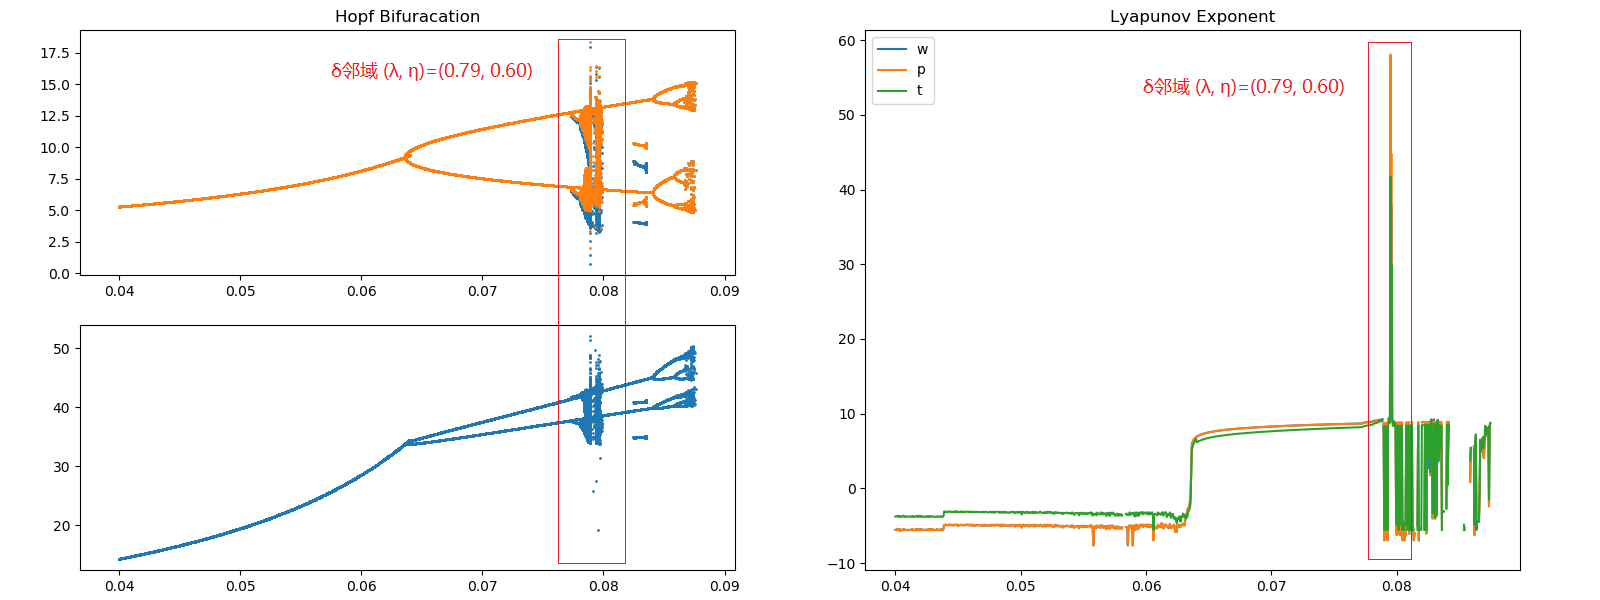
\includegraphics[width=16.5cm]{Hopf_Lyapunov_1_1.png}
    \caption{$(k_w,k_p,k_\theta;\eta,d)=(0.2,0.2,0.1,0.06,0.12)$对$\lambda$的分岔图和Lyapunov指数图}
    \label{Hopf_Lyapunov_1_1}
\end{figure}
\par 从图中可以看出,在价格调控能力相同,且处于本文假设的规模较小的市场中(只存在单一厂商和经销商),厂商开发出的直销渠道在竞争中具有绝对优势。在$\lambda\in(0,0.063)$(区间1),双方博弈处于稳定状态,然而达到均衡点时$w=p$,即经销商无利可图。这也解释了在一些规模较小的,且直销入市门槛不高的市场,电商模式代理的厂家直销可以在短时间内取代经销商的地位,从而抢得全部的市场份额。区间1中,由于绿色产品的受欢迎系数不断增大(包括政府倡导力度的作用),博弈均衡趋向于厂商提高绿色产品等级,为商品赋予更加大的附加值,同时乘机抬高价格。从$\lambda=0.063$时,系统出现二分叉,之后在$\lambda=0.079$时,出现了最大Lyapunov指数突变升高,系统在该点附近很小的领域陷入混沌,之后系统混沌程度渐进地上升,见图\ref{Hopf_Lyapunov_1_2},\ref{Hopf_Lyapunov_1_3}。
\begin{figure}[htp]
    \centering
    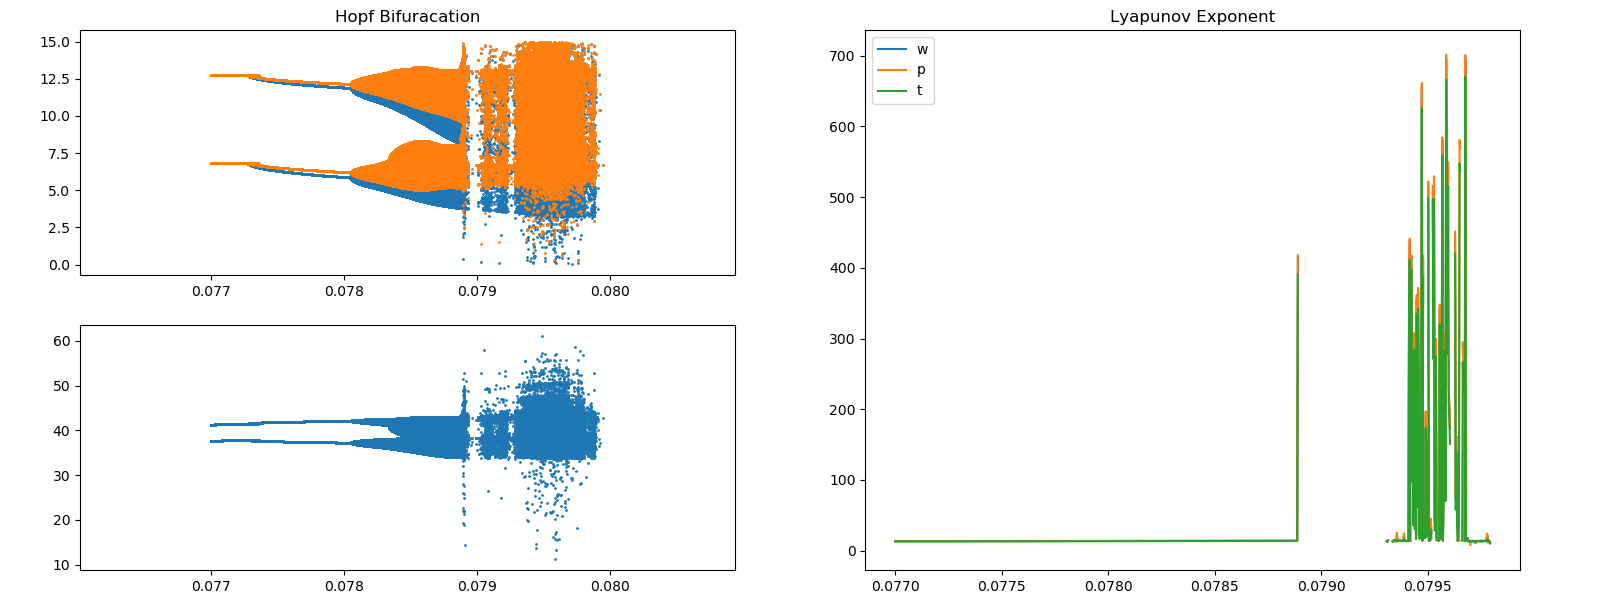
\includegraphics[width=16.5cm]{Hopf_Lyapunov_1_2.png}
    \caption{$\delta$邻域的放大分岔图}
    \label{Hopf_Lyapunov_1_2}
\end{figure}
\par 我们对该区域的现象解释为:厂商凭借技术优势创造的红利在此处消失,即由于技术创新的难度呈二次项递增(基于假设三),无法达到线性的需求增长。厂商此后最大化利益的最有效手段仍然是抢占对手——经销商的市场,使得自己保持较高的销量。同理,在$\delta$领域处,经销商重新拥有了议价能力,从而重新获得利润。
\begin{figure}[htp]
    \centering
    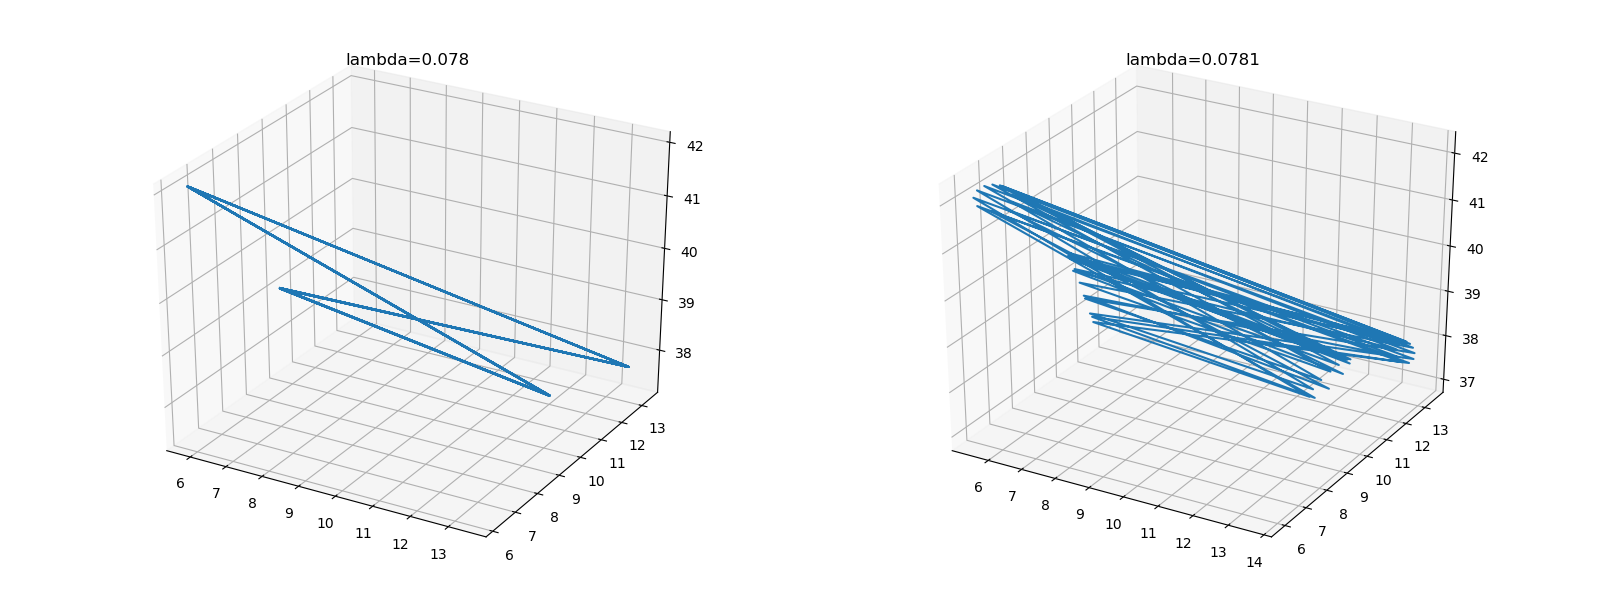
\includegraphics[width=16.5cm]{Hopf_Lyapunov_1_3.png}
    \caption{$\lambda=0.0780, 0.0781$时的混沌程度显著升高}
    \label{Hopf_Lyapunov_1_3}
\end{figure}
\subsection{讨论二:$k_w=k_p$情形下系统对$\eta$的反馈}
\par 此时我们固定了$(\lambda,d)=(0.79,0.12)$,即讨论二中平衡点,通过参数$\eta\in(0,0.08)$的模拟,得出分岔图和Lyapunov指数图\ref{Hopf_Lyapunov_2_1}:
\begin{figure}[htp]
    \centering
    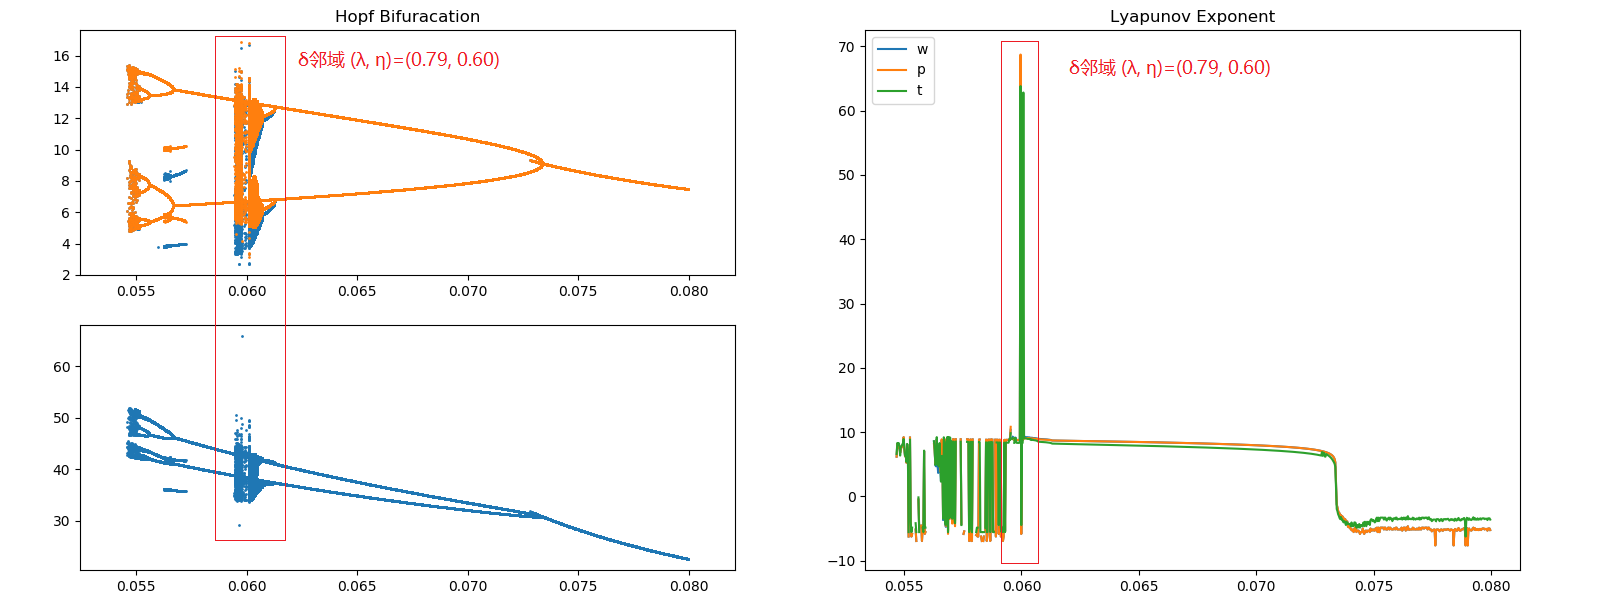
\includegraphics[width=16.5cm]{Hopf_Lyapunov_2_1.png}
    \caption{$(k_w,k_p,k_\lambda;\eta,d)=(0.2,0.2,0.1,0.79,0.12)$对$\eta$的分岔图和Lyapunov指数图}
    \label{Hopf_Lyapunov_2_1}
\end{figure}
\par 从图中我们可以总结出与讨论一相类似的结论,绿色成本系数$\eta$对价格博弈的本质性影响与系数$\lambda$相似,然而影响力更加强烈,表现在$\theta$的变化率较大。综合讨论一,我们可以知道,对于政府而言,无论是价格补贴手段(增大$\lambda$)还是生产补贴(降低$\eta$),从本文模型模拟结果来看,都存在使得系统复杂度增大,直至超过某一限度使得系统陷入混沌,即市场进入无序竞争的模式的影响。从另一角度观察,这一类的补贴手段有助于促进产业链总体向绿色的方向发展。$\delta$邻域突变现象出现的双方竞争,在许多情形下形成现实意义中的价格战,即均衡点远低于原先水平,进入一个狭小的$\delta$邻域后大部分博弈结果都趋近于极端情况,即绝大部分竞争者出场。该点发生的现象,可以作为解释所谓“O2O线上线下”价格战的机理之一。同时,同质与本文所讨论的所谓绿色供应链模型,许多创新型产品,特别是依赖于产品附加值的商品线上线下供应链所面临的调整,也可被本文所提出的解释模型所部分解答。
\subsection{讨论三:$k_w\neq k_r$情形下系统对$\lambda, \eta$的反馈}\label{sec_3_3}
\par 由讨论一和讨论二已知在博弈双方对价格的调控能力相同时,厂商具有绝对的优势取代其代理商。然而,在现实情境下,由于经销商更加贴近顾客,且其固有成本较低,导致其更加有能力快速调整价格策略。在讨论三中,我们考虑以下假设:
\par \textbf{基本假设六:}假设经销商调整市场价格的能力大于厂商调整批发价的能力$(k_w, k_p, k_\theta)=(0.15,0.35,0.1)$。
\par 在此假设下,我们首先固定$\eta=0.2$,得出$\lambda\in(0.01,0.1)$的分岔图和Lyapunov指数图\ref{Hopf_Lyapunov_3_1}:
\begin{figure}[htp]
    \centering
    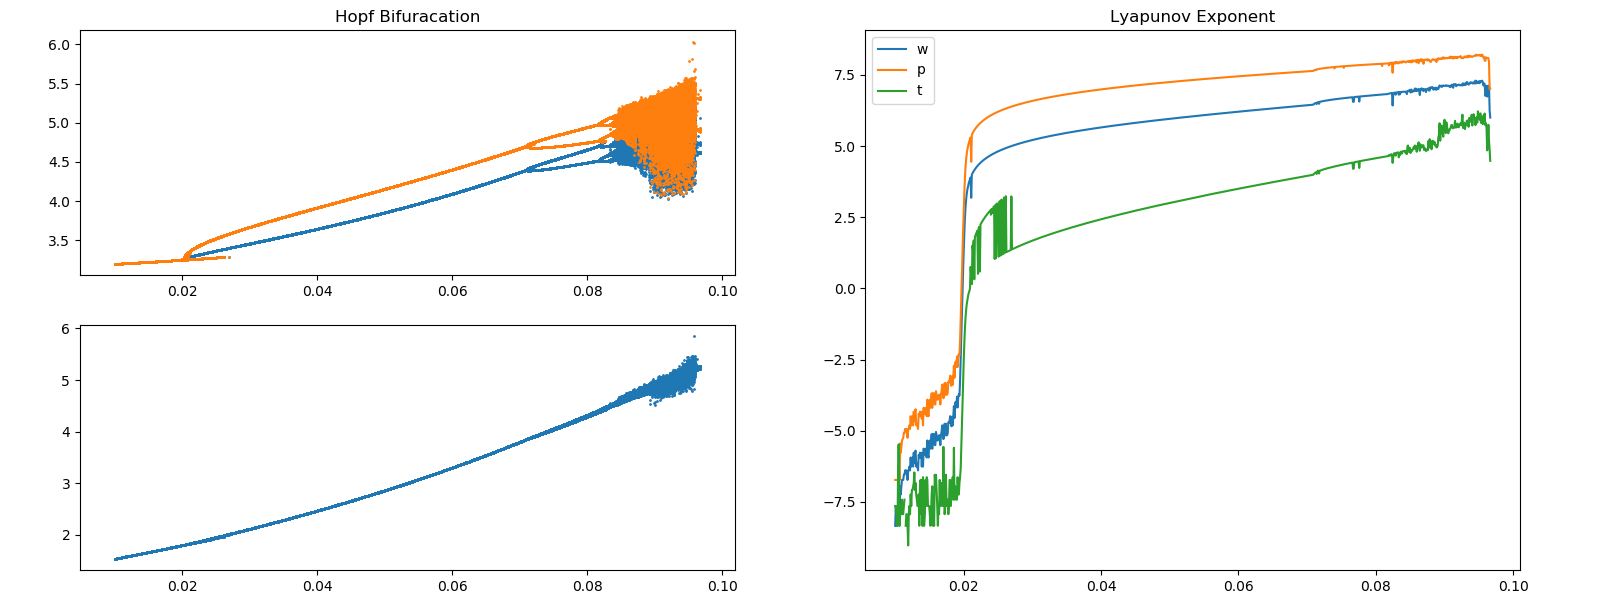
\includegraphics[width=16.5cm]{Hopf_Lyapunov_3_1.png}
    \caption{$(k_w,k_p,k_\eta;\eta,d)=(0.15,0.35,0.1,0.2,0.12)$对$\lambda$的分岔图和Lyapunov指数图}
    \label{Hopf_Lyapunov_3_1}
\end{figure}
\par 同时在$\lambda=0.04$固定时,我们得出$\eta\in(0.1, 0.5)$时的分岔图和Lyapunov指数图\ref{Hopf_Lyapunov_3_2}:
\begin{figure}[htp]
    \centering
    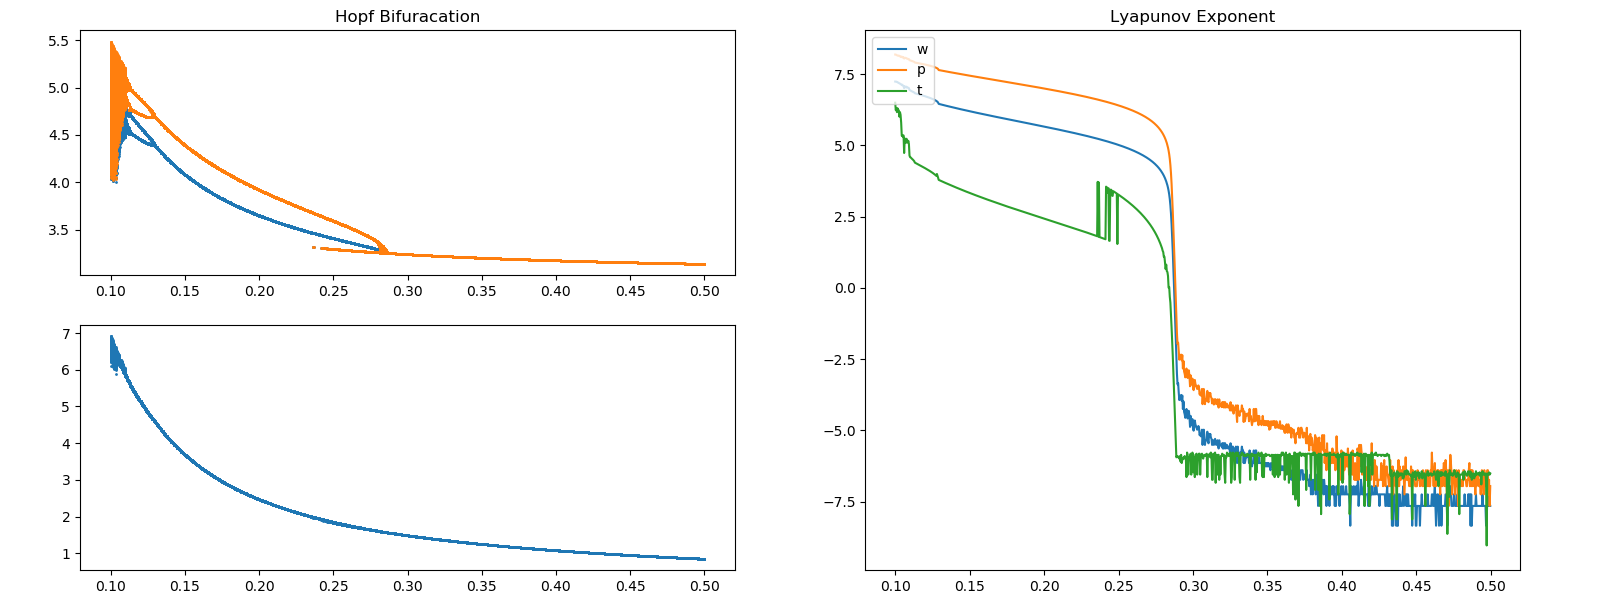
\includegraphics[width=16.5cm]{Hopf_Lyapunov_3_2.png}
    \caption{$(k_w,k_p,k_\lambda;\eta,d)=(0.15,0.35,0.1,0.04,0.12)$对$\eta$的分岔图和Lyapunov指数图}
    \label{Hopf_Lyapunov_3_2}
\end{figure}
\begin{figure}[htp]
    \centering
    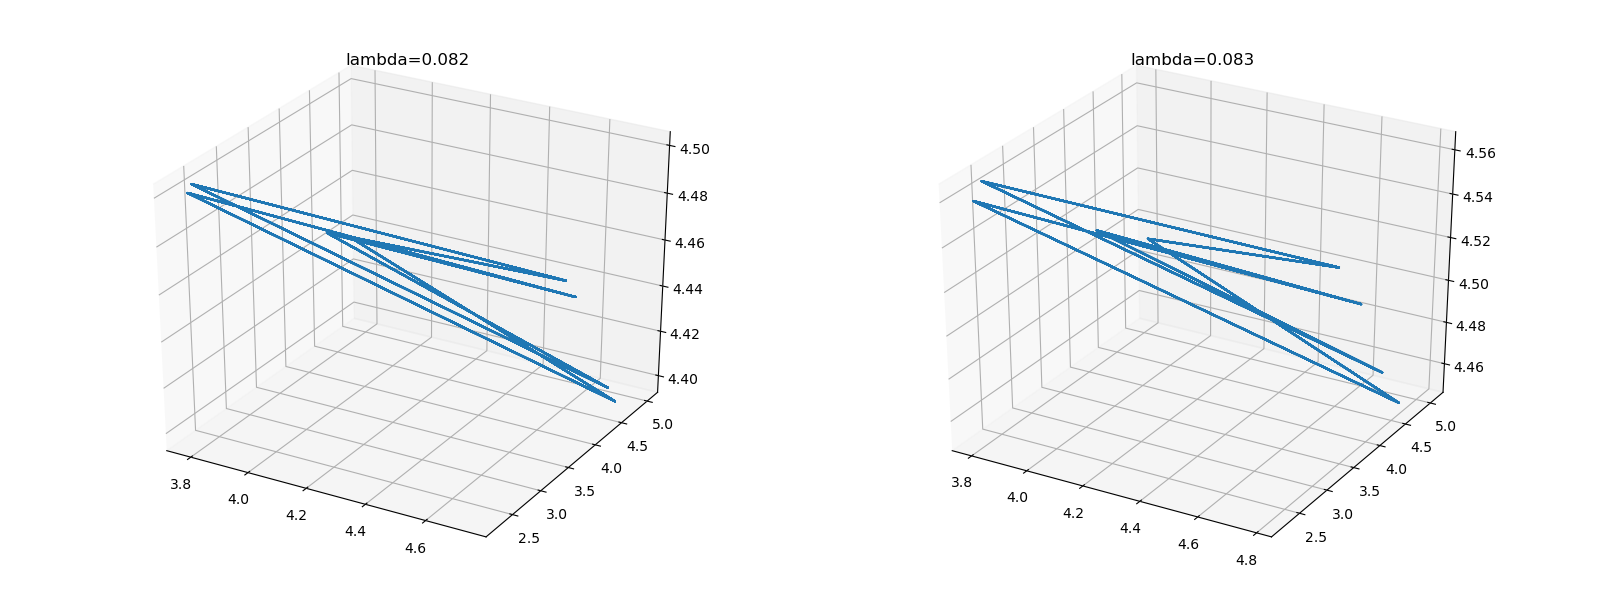
\includegraphics[width=16.5cm]{Hopf_Lyapunov_3_3.png}
    \caption{$\lambda=0.082, 0.083$时的混沌程度逐步提高}
    \label{Hopf_Lyapunov_3_3}
\end{figure}
\par 对比二者结果,我们发现,在绿色供应链初期,厂商依然垄断着市场,令零售商理论上失去了生存空间。然而,当产业链的绿色化程度逐渐加大,厂商由于承担着生产该类产品的职责,即需要投入更多的固定成本,这使得厂商实际上议价的能力减弱。图\ref{Hopf_Lyapunov_1_1}中$\lambda=0.2$,图\ref{Hopf_Lyapunov_3_2}中$\eta=0.28$这两点都出现分岔,并且分岔之后市场价高出批发价,对于零售商来说增加了利润空间。然而,此时也正是系统混沌性骤升的时刻。从Lyapunov指数图中分析,零售商所依赖的市场价格$p$的Lyapunov指数持续增加,且大于批发价格$w$。这说明了,虽然零售商此后有利可图,但是其实际风险却大于厂商。从推动绿色供应链健康发展的角度考虑,我们发现,当零售商存在利益的博弈情况下,绿色产品环保等级表现出一致性的提高。绿色等级在博弈过程中并无发生分岔,即说明了提高绿色等级是双方利益最大化的一致性目标。
\section{结论}
\par 总结第三、四节的数学分析和数值模拟结果,我们从厂商、零售商、政府干预这三个角度和绿色产业链发展的关系,总结其各自在绿色双渠道供应链中的处境以及战略:
\begin{itemize}
    \item \textbf{对于厂商而言},其增加的直销渠道对于零售商有着极大的取代能力,处于绝对优势地位。然而对比\ref{sec_3_1}和\ref{sec_3_3}的模拟结果,我们可以发现该处境使得系统出现的混沌更加显著。
    \item \textbf{对于零售商而言},其处于定价方面的劣势地位,在静态博弈假设下无法胜出。然而,在动态博弈中,由于其贴近市场的优势,以及其自身的灵活性,在调节能力方面的优势可以为其争取利润空间(\ref{sec_3_3})。同时,产品绿色等级的提升也有助于其争取自身利润(\ref{sec_3_3})。因此,经销商的利益应该与推动产品环保等级提升一致。同时,基于\cite{2018Huang}\cite{2018Li}的研究,零售商的利润空间同时可以被加入到其功利的考虑,以为其自身获取利益。
    \item \textbf{政府干预措施},特别是对于绿色产品的消费和生产补贴,事实上有助于厂商主动提高该产品的绿色等级。然而,在激励力度达到某一程度时,该效应同时影响到了市场的稳定程度。模拟结果表面,较大力度的激励措施,会使厂商在决定自身产品绿色等级的决策中出现分岔(\ref{sec_3_1}),即对激励作用本身产生负面影响,且在激励力度过于强烈时,该决策将陷入混沌。只有在零售商与厂商有效竞争(非厂商独占),以及激励手段强度在合理范围内,产品的环保等级才能持续增长,同时保持市场稳定运行(\ref{sec_3_3})。
\end{itemize}
\par

\begin{thebibliography}{1}
\bibitem{2005Beamon} Beamon, B.M. SCI ENG ETHICS (2005) 11: 221. https://doi.org/10.1007/s11948-005-0043-y
\bibitem{2009Wang} 王虹, 周晶. 不同价格模式下的双渠道供应链决策研究[J]. 中国管理科学, 2009, V17(6):84-90.
\bibitem{2012Sheu} Jiuh-Biing Sheu, Yenming J. Chen, Impact of government financial intervention on competition among green supply chains, \emph{International Journal of Production Economics}, Volume 138, Issue 1, 2012, Pages 201-213, ISSN 0925-5273, https://doi.org/10.1016/j.ijpe.2012.03.024.
\bibitem{2012Ghosh} Debabrata Ghosh, Janat Shah, A comparative analysis of greening policies across supply chain structures, \emph{International Journal of Production Economics}, Volume 135, Issue 2, 2012, Pages 568-583, ISSN 0925-5273, https://doi.org/10.1016/j.ijpe.2011.05.027.
\bibitem{2015Zhang} Fang Zhang, Junhai Ma, Research on the complex features about a dual-channel supply chain with a fair caring retailer, \emph{Communications in Nonlinear Science and Numerical Simulation}, Volume 30, Issues 1–3, 2016, Pages 151-167, ISSN 1007-5704, https://doi.org/10.1016/j.cnsns.2015.06.009.
\bibitem{2016Wang} Cong Wang, De-li Yang, and Zhao Wang, “Comparison of Dual-Channel Supply Chain Structures: E-Commerce Platform as Different Roles,” \emph{Mathematical Problems in Engineering}, vol. 2016, Article ID 3831624, 10 pages, 2016. https://doi.org/10.1155/2016/3831624.
\bibitem{2016Li} Qing-Hua Li, Bo Li, Dual-channel supply chain equilibrium problems regarding retail services and fairness concerns, \emph{Applied Mathematical Modelling}, Volume 40, Issues 15–16, 2016, Pages 7349-7367, ISSN 0307-904X, https://doi.org/10.1016/j.apm.2016.03.010.
\bibitem{2017Zhao} Jing Zhao, Xiaorui Hou, Yunlian Guo, Jie Wei, Pricing policies for complementary products in a dual-channel supply chain, \emph{Applied Mathematical Modelling}, Volume 49, 2017, Pages 437-451, ISSN 0307-904X, https://doi.org/10.1016/j.apm.2017.04.023.
\bibitem{2017Tang} 唐兴巧, 蒲新会, 蔡成松. 一类双渠道供应链博弈模型的分岔与混沌分析[J]. 温州大学学报(自然科学版), 2017(2).
\bibitem{2018Xie} Xie Fengqin, Nie Qixuan, Yu Hongfei, Inventory Strategy of Dual-Channel Supply Chain from Manufacturer's Perspective, \emph{International Journal of Management and Fuzzy Systems}. Vol. 4, No. 2, 2018, pp. 29-34. doi: 10.11648/j.ijmfs.20180402.14
\bibitem{2018Arshad} Arshad, M.; Khalid, Q.S.; Lloret, J.; Leon, A. An Efficient Approach for Coordination of Dual-Channel Closed-Loop Supply Chain Management. \emph{Sustainability} 2018, 10, 3433.
\bibitem{2018Wang} Yuyan Wang, Zhaoqing Yu , Liang Shen (2019) Study on the decision-making and coordination of an e-commerce supply chain with manufacturer fairness concerns, \emph{International Journal of Production Research}, 57:9, 2788-2808, DOI: 10.1080/00207543.2018.1500043
\bibitem{2018Li} 李盈盈,张雪梅,陈媛媛等.不同价格模式下的双渠道供应链决策研究[J].阜阳师范学院学报(自然科学版),2018,35(3):21-27.DOI:10.14096/j.cnki.cn34-1069/n/1004-4329(2018)03-021-07.
\bibitem{2018Zhang} 张芳, 马小林. 双渠道闭环供应链博弈模型的复杂性分析[J]. 天津工业大学学报, 2018, v.37;No.180(03):78-84.
\bibitem{2018Huang} Huang Yi-min, Li Qiu-xiang, and Zhang Yu-hao, “The Complexity Analysis for Price Game Model of Risk-Averse Supply Chain Considering Fairness Concern,” \emph{Complexity}, vol. 2018, Article ID 9216193, 15 pages, 2018. https://doi.org/10.1155/2018/9216193.
\bibitem{2018Qiu-Xiang} Li Qiu-xiang, Zhang Yu-hao, and Huang Yi-min, “The Complexity Analysis in Dual-Channel Supply Chain Based on Fairness Concern and Different Business Objectives,” \emph{Complexity}, vol. 2018, Article ID 4752765, 13 pages, 2018. https://doi.org/10.1155/2018/4752765.
\bibitem{2018Sinayi} Mohammadreza Sinayi, Morteza Rasti-Barzoki, A game theoretic approach for pricing, greening, and social welfare policies in a supply chain with government intervention, \emph{Journal of Cleaner Production}, Volume 196, 2018, Pages 1443-1458, ISSN 0959-6526, https://doi.org/10.1016/j.jclepro.2018.05.212.
\bibitem{2018Rahami} Kavian Rahmani, Mohammad Yavari, Pricing policies for a dual-channel green supply chain under demand disruptions, \emph{Computers \& Industrial Engineering}, Volume 127, 2019, Pages 493-510, ISSN 0360-8352, https://doi.org/10.1016/j.cie.2018.10.039.
\bibitem{2019Pathak} Pathak, U., Kant, R. , Shankar, R. OPSEARCH (2019). https://doi.org/10.1007/s12597-019-00421-z
\bibitem{2019Giri} B.C. Giri, S.K. Dey, Game theoretic analysis of a closed-loop supply chain with backup supplier under dual channel recycling, \emph{Computers \& Industrial Engineering}, Volume 129, 2019, Pages 179-191, ISSN 0360-8352, https://doi.org/10.1016/j.cie.2019.01.035. 
\bibitem{2019Hosseini-Motlagh} Seyyed-Mahdi Hosseini-Motlagh, Mina Nouri-Harzvili, Tsan-Ming Choi, Samira Ebrahimi, Reverse supply chain systems optimization with dual channel and demand disruptions: Sustainability, CSR investment and pricing coordination, \emph{Information Sciences}, Volume 503, 2019, Pages 606-634, ISSN 0020-0255, https://doi.org/10.1016/j.ins.2019.07.021.
\bibitem{2019Dai} Lufeng Dai, Xifu Wang, Xiaoguang Liu, and Lai Wei, “Pricing Strategies in Dual-Channel Supply Chain with a Fair Caring Retailer,” \emph{Complexity}, vol. 2019, Article ID 1484372, 23 pages, 2019. https://doi.org/10.1155/2019/1484372.
\bibitem{2019Qiu-Xiang1} Li, Q.; Chen, X.; Huang, Y. The Stability and Complexity Analysis of a Low-Carbon Supply Chain Considering Fairness Concern Behavior and Sales Service. \emph{Int. J. Environ. Res. Public Health} 2019, 16, 2711.
\bibitem{2019Qiu-Xiang2} Li, Q.; Shi, M.; Deng, Q.; Huang, Y.-M. The Complexity Entropy Analysis of a Supply Chain System Considering Recovery Rate and Channel Service. \emph{Entropy} 2019, 21, 659.
\bibitem{2019Aslani} Amin Aslani, Jafar Heydari, Transshipment contract for coordination of a green dual-channel supply chain under channel disruption, \emph{Journal of Cleaner Production}, Volume 223, 2019, Pages 596-609, ISSN 0959-6526, https://doi.org/10.1016/j.jclepro.2019.03.186.

\end{thebibliography}
\end{document}